\subsubsection{\stid{6.01} LANL ATDM Data and Visualization} 

\paragraph{Overview} 
The LANL ATDM Data and Visualization project develops scalable
systems software for the generation, analysis, and management of data
produced by ECP applications. This project is essential for ECP because
of the volume of data exascale applications will generate.

\paragraph{Key Challenges}
Interfacing to a large number of ECP application with the Cinema software and the management of the volumous data from these applications.

\paragraph{Solution Strategy}
To provide turn-key visualizationsoftware based on cinema for post and in situ application data processing.
\paragraph{Recent Progress}
\begin{figure}[htb]
	\centering
	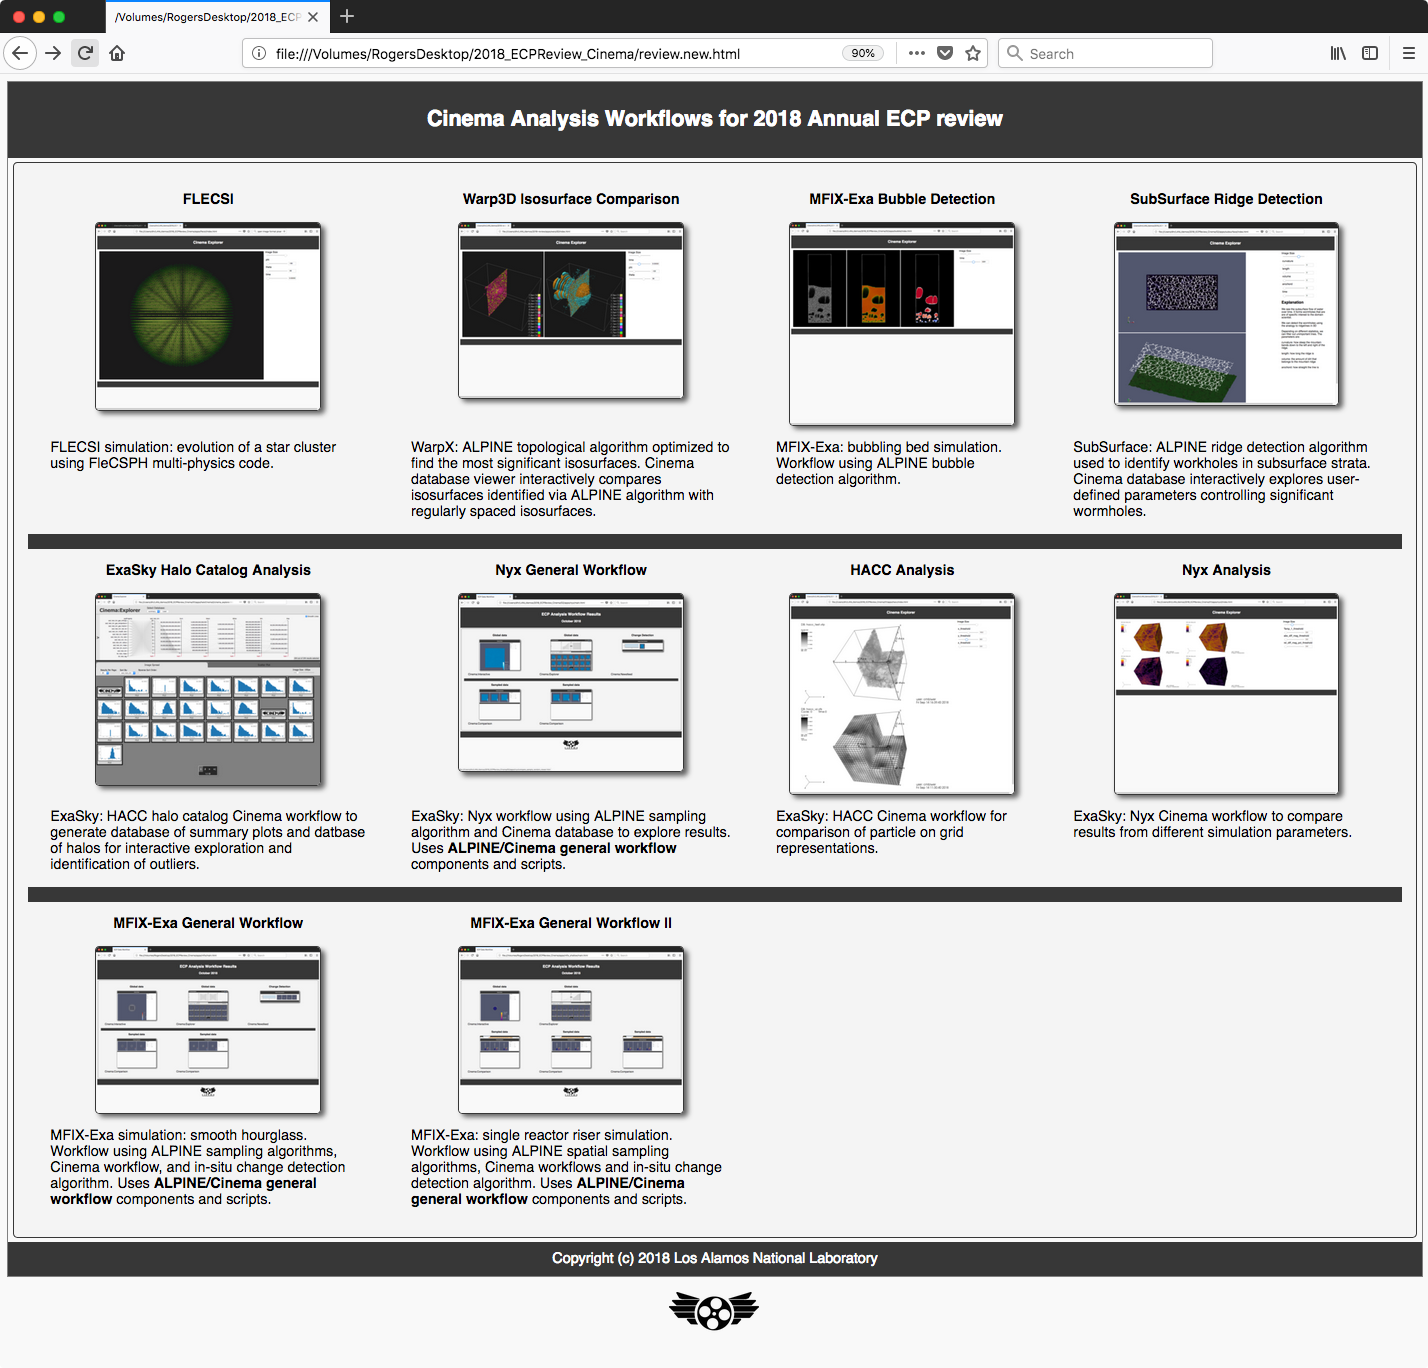
\includegraphics[width=5in]{projects/2.3.6-NNSA/2.3.6.01-LANL-ATDM/ECPReviewScreenshot.png}
	\caption{
        Screen capture of a browser-based set of Cinema viewers 
        for a set of ECP datasets. We ran a variety of ALPINE algorithms
        extracted relevant data features, and then output 
        results as Cinema databases visualized in
        a variety of ways, including comparison views, database
        explorers, and change detection.
    }
\end{figure}

Recent Cinema work has focused on development of capability
and workflows for change detection in-situ data analysis artifacts. These
promote new ways of analyzing ECP data, including
automated and assisted analysis. New capabilities provide 
scientists more options in analyzing and exploring the results of large
simulations by provide a workflow that 1) detects features in-situ, 2)
captures data artifacts in Cinema databases, 3) promotes
post-hoc analysis of the data, and 4)
provides data viewers that allow interactive, structured exploration of the
resulting artifacts. In our most recent milestone, we ran
ALPINE algorithms and Cinema viewer creation workflows on a variety of
ECP and ATDM simulation results to demonstrate integration with applications
and progress in focusing on ECP application needs.
This overall workflow provides a
flexible method of applying new algorithms to the analysis and visualization
of extreme scale data.

\paragraph{Next Steps}
%\textit{Describe what you are working on next.}
Cinema is identifying new application workflows that can be reasonably made
efficient and new analysis methods to apply efficiently for cinema
users.
